\chapter{Resultados}
En este capítulo se presentan los resultados obtenidos tras el entrenamiento y evaluación de los modelos de redes neuronales implementados en Keras y PyTorch, así como una comparación de los resultados de las evaluaciónes. Además, se incluyen los resultados de las pruebas comparativas realizadas entre la nariz electrónica entrenada y el agente canino de la Guardia Civil encargado en la detección de drogas.

\section{Resultados de redes neuronales}
Tras el entrenamiento, se evalúa el modelo en el conjunto de prueba para garantizar que los resultados no sufren de sobreajuste. El rendimiento se visualiza mediante curvas de aprendizaje (Accuracy y Loss), con una precisión (Accuracy) del 77.78\%, para verificar la convergencia, como se observa en la Figura~\ref{fig:curvas_entrenamiento_Keras} y una matriz de confusión para observar cómo clasifica el sistema las muestras ``Buenas'' y ``Malas'' reales frente a las predichas. Dicha matriz puede verse en la Figura~\ref{fig:matriz_confusion_Keras}.
\par

\begin{figure}[H]
    \centering
    \shadowbox{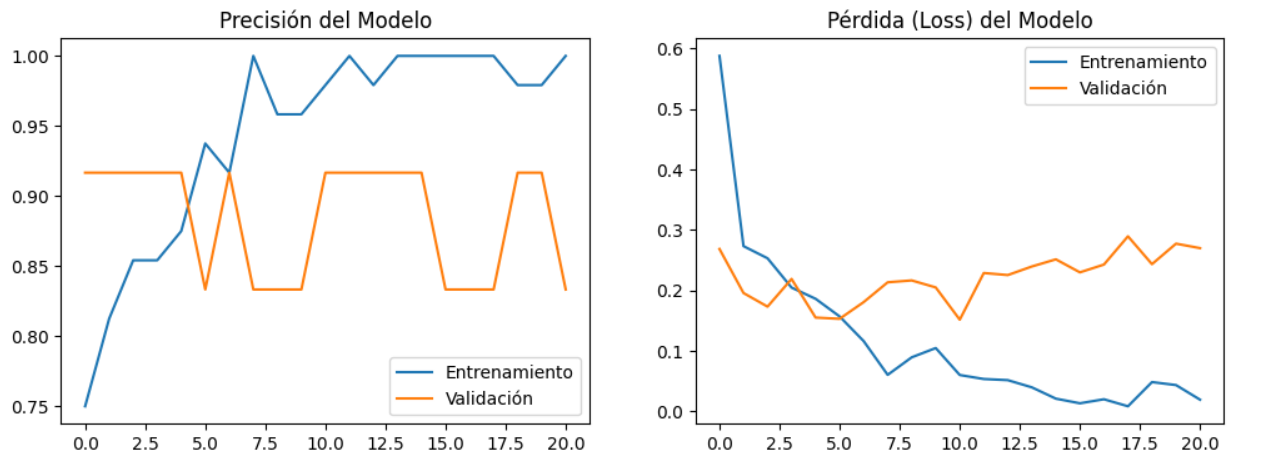
\includegraphics[width=0.8\textwidth]{pictures/Curvas_entrenamiento_keras.png}}
    \caption{Curvas de precisión (Accuracy) y pérdida (Loss) durante el entrenamiento y validación del modelo en Keras.}\label{fig:curvas_entrenamiento_Keras}
\end{figure}

\begin{figure}[H]
    \centering
    \shadowbox{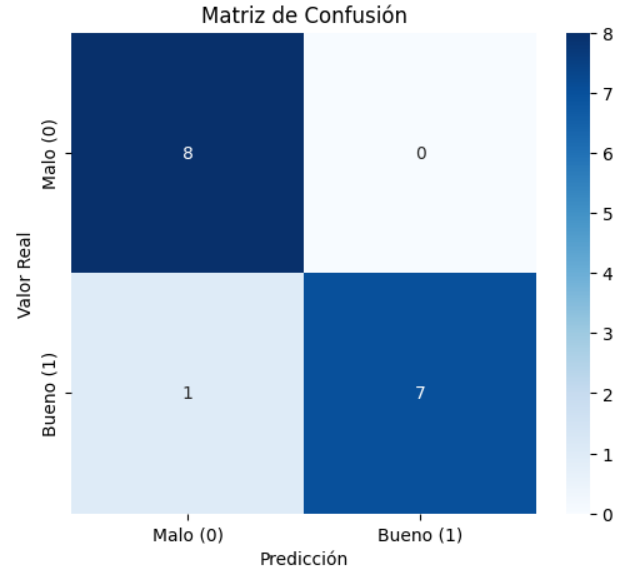
\includegraphics[width=0.5\textwidth]{pictures/Matriz_confusion_keras.png}}
    \caption{Matriz de confusión del modelo entrenado en Keras.}\label{fig:matriz_confusion_Keras}
\end{figure}

Tras completar las épocas de entrenamiento, el modelo fue evaluado con el conjunto de prueba (datos no vistos). Se generaron curvas de Loss y Accuracy, que pueden verse en la Figura~\ref{fig:curvas_entrenamiento_PyTorch}, para verificar la estabilidad del aprendizaje y una Matriz de Confusión, vease en la figura~\ref{fig:matriz_confusion_PyTorch}, para analizar el balance entre falsos positivos y falsos negativos.

\begin{figure}[H]
    \centering
    \shadowbox{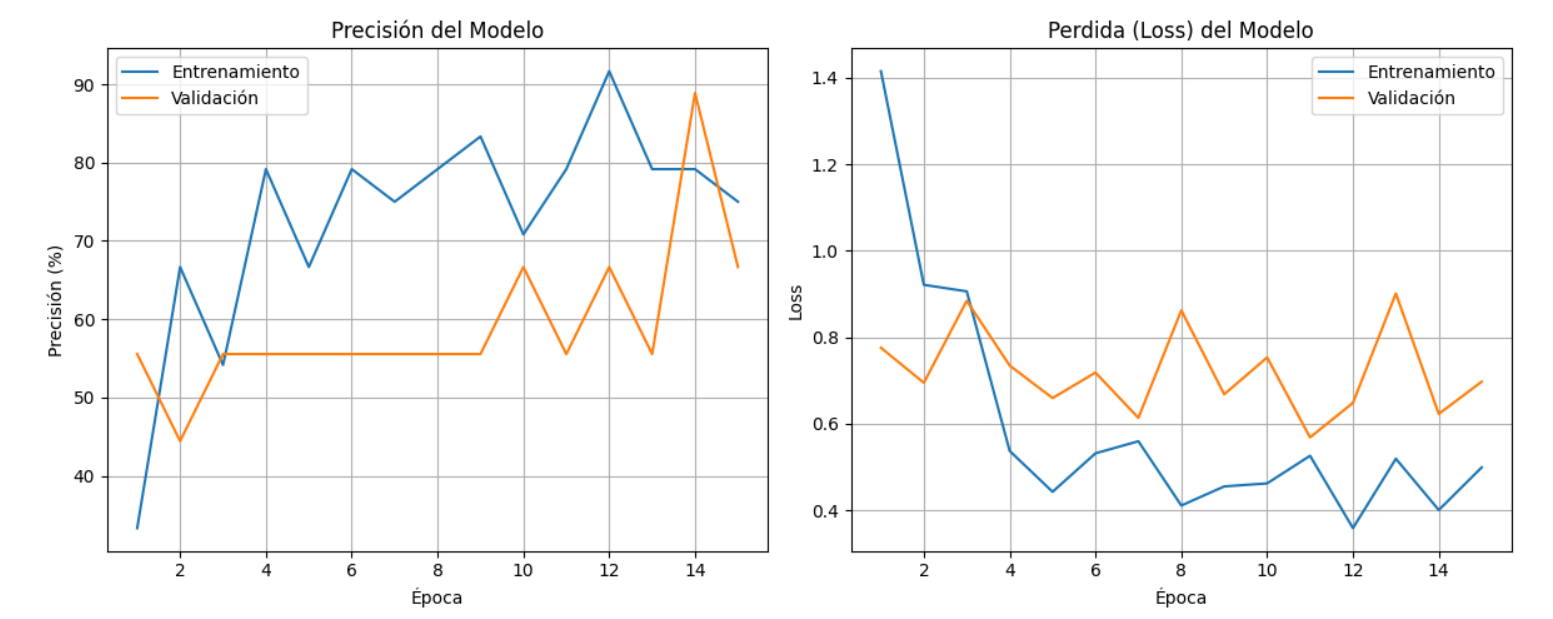
\includegraphics[width=0.9\textwidth]{pictures/Curvas_entrenamiento_pytorch.png}}
    \caption{Curvas de precisión (Accuracy) y pérdida (Loss) durante el entrenamiento y validación del modelo en PyTorch.}\label{fig:curvas_entrenamiento_PyTorch}
\end{figure}

\begin{figure}[H]
    \centering
    \shadowbox{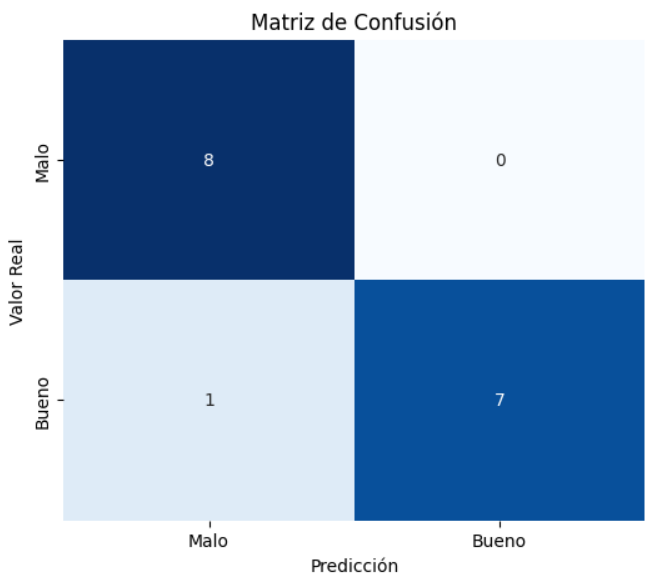
\includegraphics[width=0.7\textwidth]{pictures/Matriz_confusion_pytorch.png}}
    \caption{Matriz de confusión del modelo entrenado en PyTorch.}\label{fig:matriz_confusion_PyTorch}
\end{figure}

\section{Resultados de pruebas comparativas}